\documentclass[11pt,a4paper,twocolumn]{article}

\usepackage[utf8]{inputenc}
\usepackage[T1]{fontenc}
\usepackage{lmodern}
\usepackage{amsmath,amssymb,amsfonts}
\usepackage{graphicx}
\usepackage{xcolor}
\usepackage{hyperref}
\usepackage{booktabs}
\usepackage{enumitem}
\usepackage{float}
\usepackage{caption}
\usepackage{algorithm}
\usepackage{algpseudocode}
\usepackage{listings}
\usepackage[margin=2cm]{geometry}
\usepackage{titlesec}
\usepackage{cite}
\usepackage{url}
\usepackage{array}
\usepackage{tabularx}
\usepackage{stfloats}
\usepackage{placeins}  % FloatBarrier

\definecolor{linkblue}{HTML}{2563EB}
\definecolor{codegray}{HTML}{F1F5F9}
\definecolor{codetext}{HTML}{1E293B}

\hypersetup{
    colorlinks=true, linkcolor=linkblue,
    citecolor=linkblue, urlcolor=linkblue,
    pdfauthor={Seo Mk},
    pdftitle={PoRE: Policy-governed Resolution Engine},
}

\lstset{
    backgroundcolor=\color{codegray},
    basicstyle=\ttfamily\footnotesize\color{codetext},
    breaklines=true, frame=single,
    rulecolor=\color{gray!30}, numbers=none,
}

\titleformat{\section}{\large\bfseries}{\thesection.}{0.5em}{}
\titleformat{\subsection}{\normalsize\bfseries}{\thesubsection}{0.5em}{}

% ══════════════════════════════════════════════════════════
\begin{document}

\twocolumn[
\begin{@twocolumnfalse}
\begin{center}
{\LARGE\bfseries PoRE: Policy-governed Resolution Engine\\[6pt]}
{\large Decentralized Source Curation and Deterministic Safety\\
for Prediction Market Resolution\\[12pt]}
{\normalsize Seo Mk\\[4pt]}
{\small Version 1.0 --- February 2026}
\end{center}
\vspace{6pt}

\begin{abstract}
\noindent Prediction markets have emerged as powerful mechanisms for aggregating information, with platforms like Polymarket surpassing \$237M in single-market volume. However, their resolution mechanisms remain critically fragile. Current approaches---most notably UMA Protocol's Optimistic Oracle---delegate final resolution to token-weighted voting, creating structural vulnerabilities where a small number of large token holders can dictate outcomes irrespective of evidence quality. We document three high-profile resolution failures totaling over \$247M in affected volume.

We present \textbf{PoRE (Policy-governed Resolution Engine)}, a middleware protocol introducing two innovations: (1)~a \emph{deterministic policy engine} that mathematically evaluates whether automatic resolution is safe, producing explicit \textsc{hold} verdicts with auditable violation reports; and (2)~a \emph{Decentralized Source Curation} mechanism that replaces direct outcome voting with token-weighted evidence validation, shifting the manipulation vector from 1-bit outcome corruption to $N$-dimensional evidence ecosystem subversion. In replay simulations of all three documented failures, PoRE correctly produced \textsc{hold} verdicts.
\end{abstract}
\vspace{8pt}
\end{@twocolumnfalse}
]

% ═══════════════════════════════════════════════════
\section{Introduction}

Prediction markets function as decentralized information aggregation systems where participants express probabilistic beliefs about future events through financial positions~\cite{wolfers2004prediction}. However, a prediction market is only as reliable as its \emph{resolution mechanism}. A corrupted resolution constitutes a direct wealth transfer from honest participants to manipulators.

The current dominant architecture follows a pattern: (1)~a proposer asserts the outcome, (2)~a challenge window allows disputes, and (3)~if disputed, token-weighted voting determines the final outcome. This assumes honest behavior because dishonest voting degrades ecosystem value. We demonstrate this assumption fails when the value at stake exceeds expected token value loss, and when low voter participation amplifies whale influence.

PoRE introduces a \emph{deterministic, non-manipulable safety layer}. Rather than asking ``What is the answer?'', PoRE asks ``\textbf{Is it safe to auto-resolve?}'' Furthermore, we propose \textbf{Decentralized Source Curation}---token holders vote on which evidence sources are valid, and an AI policy engine evaluates the curated evidence deterministically.

% ═══════════════════════════════════════════════════
\section{Problem Statement}

\subsection{The Resolution Trilemma}

Prediction market resolution faces a trilemma among \emph{decentralization}, \emph{accuracy}, and \emph{speed} (Figure~\ref{fig:trilemma}). Existing systems optimize for decentralization~+~speed (accepting accuracy risk). PoRE shifts the curve: auto-resolving clear cases (speed), escalating ambiguous ones (accuracy), without central authority (decentralization).

\begin{figure}[h]
    \centering
    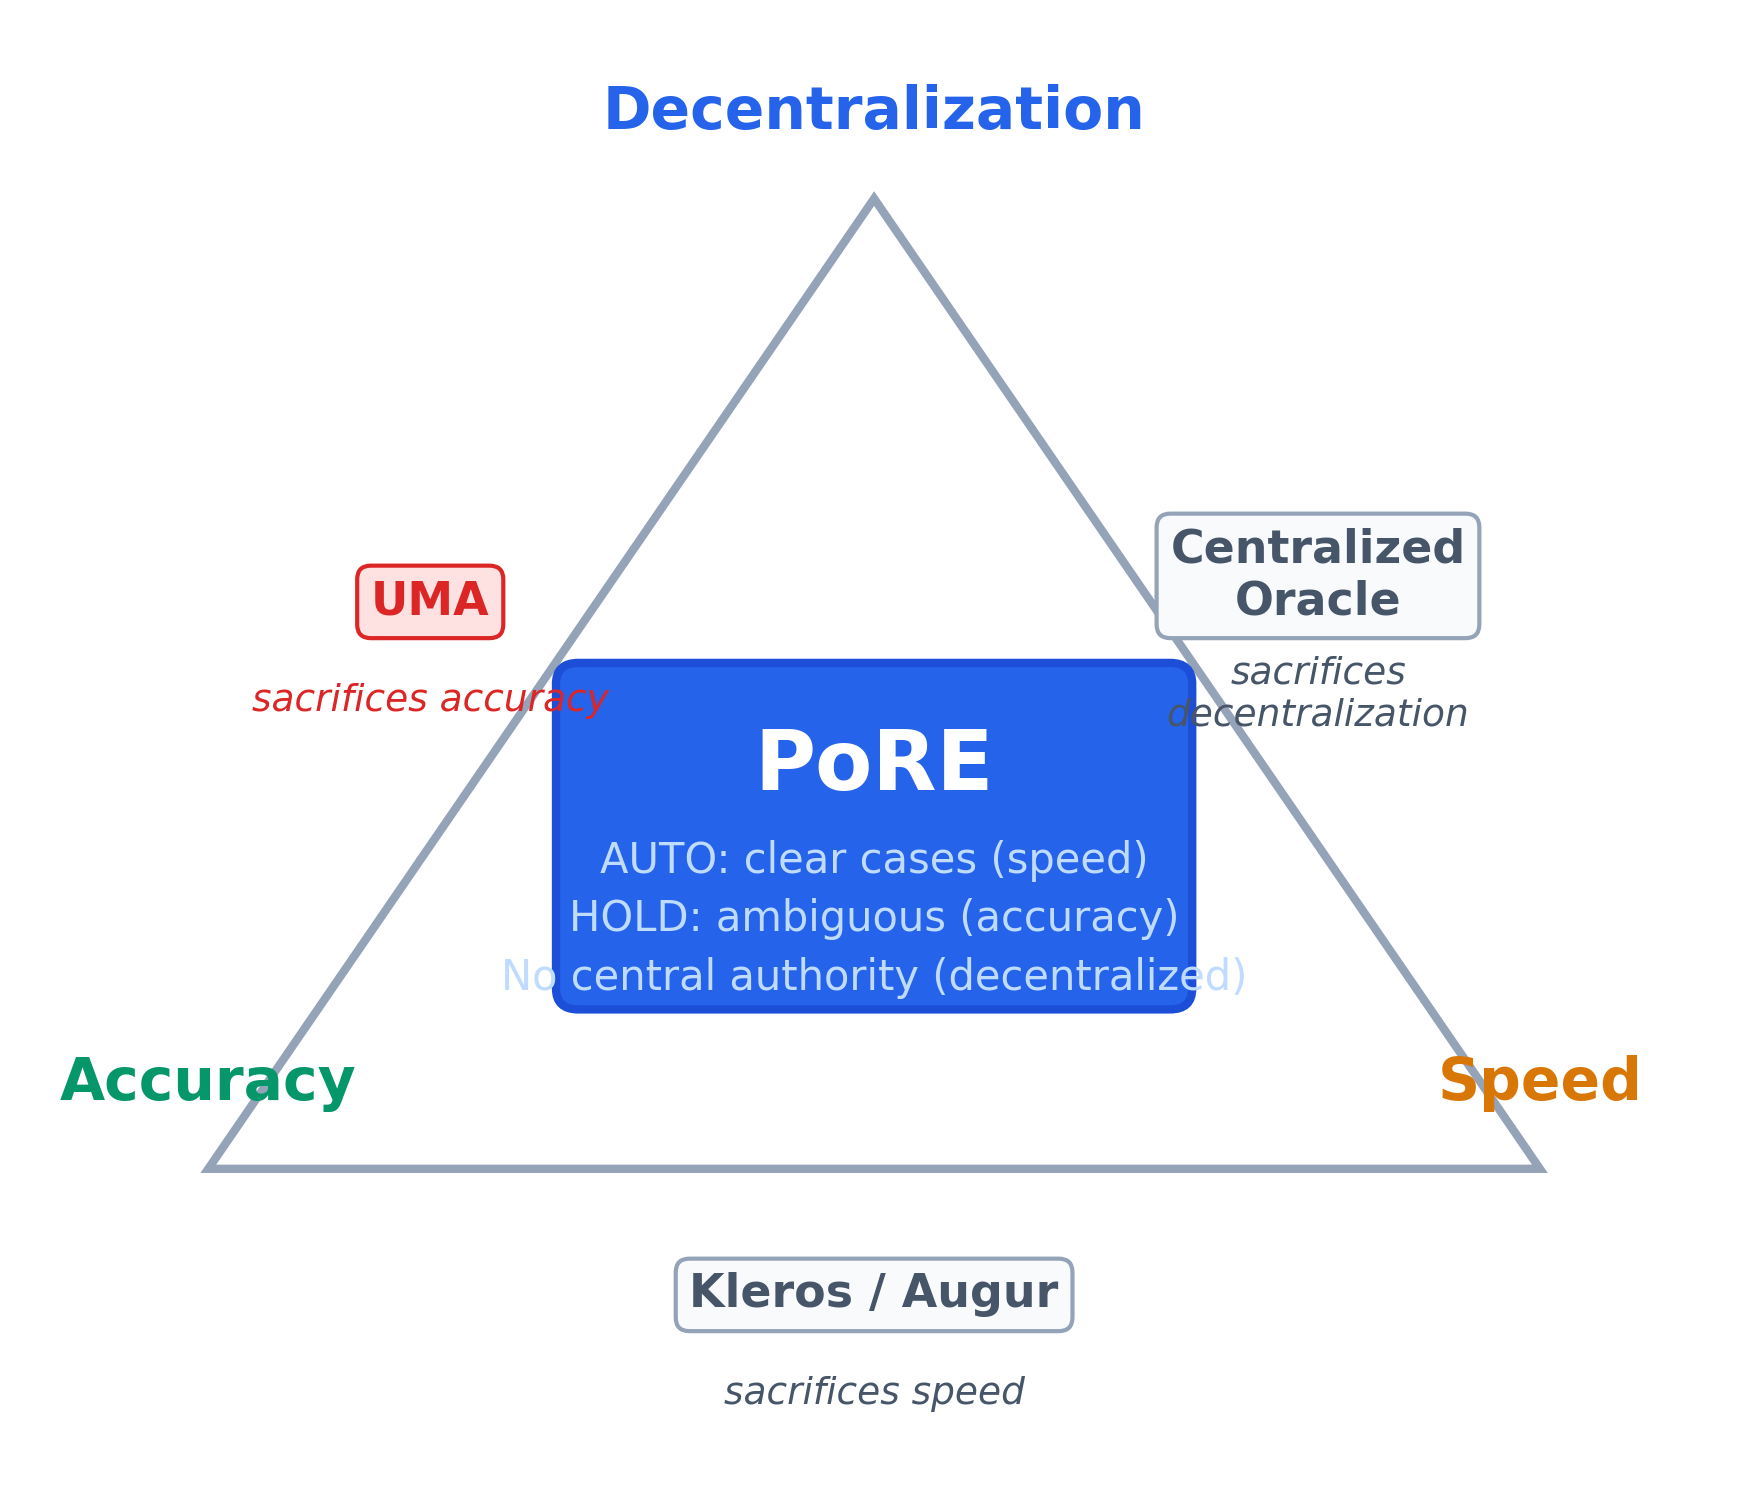
\includegraphics[width=0.85\columnwidth]{diagrams/fig6_trilemma.png}
    \caption{Resolution trilemma. PoRE uses conditional routing (\textsc{auto}/\textsc{hold}) to approach all three vertices.}
    \label{fig:trilemma}
\end{figure}

\subsection{Structural Vulnerabilities}

The UMA Optimistic Oracle~\cite{uma2020} operates through proposal, challenge, and DVM voting. We identify three vulnerabilities:

\textbf{V1: Plutocratic determination.} With ${\sim}120$M UMA supply and 10--20\% participation, a holder of 5M tokens controls 20--40\% of effective voting power.

\textbf{V2: Economic misalignment.} The security condition requires:
\begin{equation}
    C_{\text{manip}} > P_{\text{manip}}
    \label{eq:security}
\end{equation}
For the Ukraine case (\$7M market):
\begin{align}
    C &\approx 5\% \times \$10\text{M} = \$500\text{K} \nonumber \\
    P &\approx \$1\text{M to } \$5\text{M} \nonumber \\
    P &> C \implies \text{manipulation is rational}
    \label{eq:cost}
\end{align}

\textbf{V3: Semantic ambiguity.} Natural language criteria create interpretation gaps (``suit'' vs.\ ``blazer'').

\subsection{Documented Failures}

Table~\ref{tab:failures} summarizes three cases totaling \$247M+ in affected volume.

\begin{table}[h]
\centering
\caption{Documented resolution failures.}
\label{tab:failures}
\footnotesize
\begin{tabularx}{\columnwidth}{@{}Xrl@{}}
\toprule
\textbf{Case} & \textbf{Vol.} & \textbf{Exploit} \\
\midrule
Ukraine mineral deal & \$7M & Whale 25\% \\
Zelenskyy suit & \$237M & Ambiguity \\
Fort Knox gold & \$3.5M & UI disabled \\
\bottomrule
\end{tabularx}
\end{table}

% ═══════════════════════════════════════════════════
\section{Related Work}

\textbf{Chainlink}~\cite{chainlink2021} provides decentralized oracle networks optimized for objective numerical data, not subjective events. \textbf{UMA}~\cite{uma2020} is efficient for uncontroversial resolutions but degenerates to plutocratic voting. \textbf{Kleros}~\cite{kleros2017} uses random juries but introduces latency. \textbf{Augur~v2}~\cite{augur2015} uses escalating bonds, exploitable by well-funded attackers.

PoRE is a \textbf{middleware safety layer}:
\[
\text{Sources} \to \boxed{\text{PoRE}} \to
\begin{cases}
\textsc{auto} & \text{resolve} \\
\textsc{hold} & \text{escalate}
\end{cases}
\]

% ═══════════════════════════════════════════════════
\section{System Architecture}

\subsection{Five-Layer Design}

PoRE consists of five layers (Figure~\ref{fig:arch}):
\begin{enumerate}[nosep]
    \item \textbf{Evidence Collection} (pluggable): on-chain feeds, APIs.
    \item \textbf{Source Curation} (decentralized): token-weighted validation.
    \item \textbf{AI Deliberation} (probabilistic): proposer/challenger.
    \item \textbf{Policy Engine} (deterministic): 8 hard safety rules.
    \item \textbf{On-chain Recording} (immutable): verdict hashes.
\end{enumerate}

The design principle is \emph{separation of trust domains}: humans curate (L1--2), AI interprets (L3), code evaluates (L4), blockchain records (L5). No single layer has complete authority.

\begin{figure*}[!htbp]
    \centering
    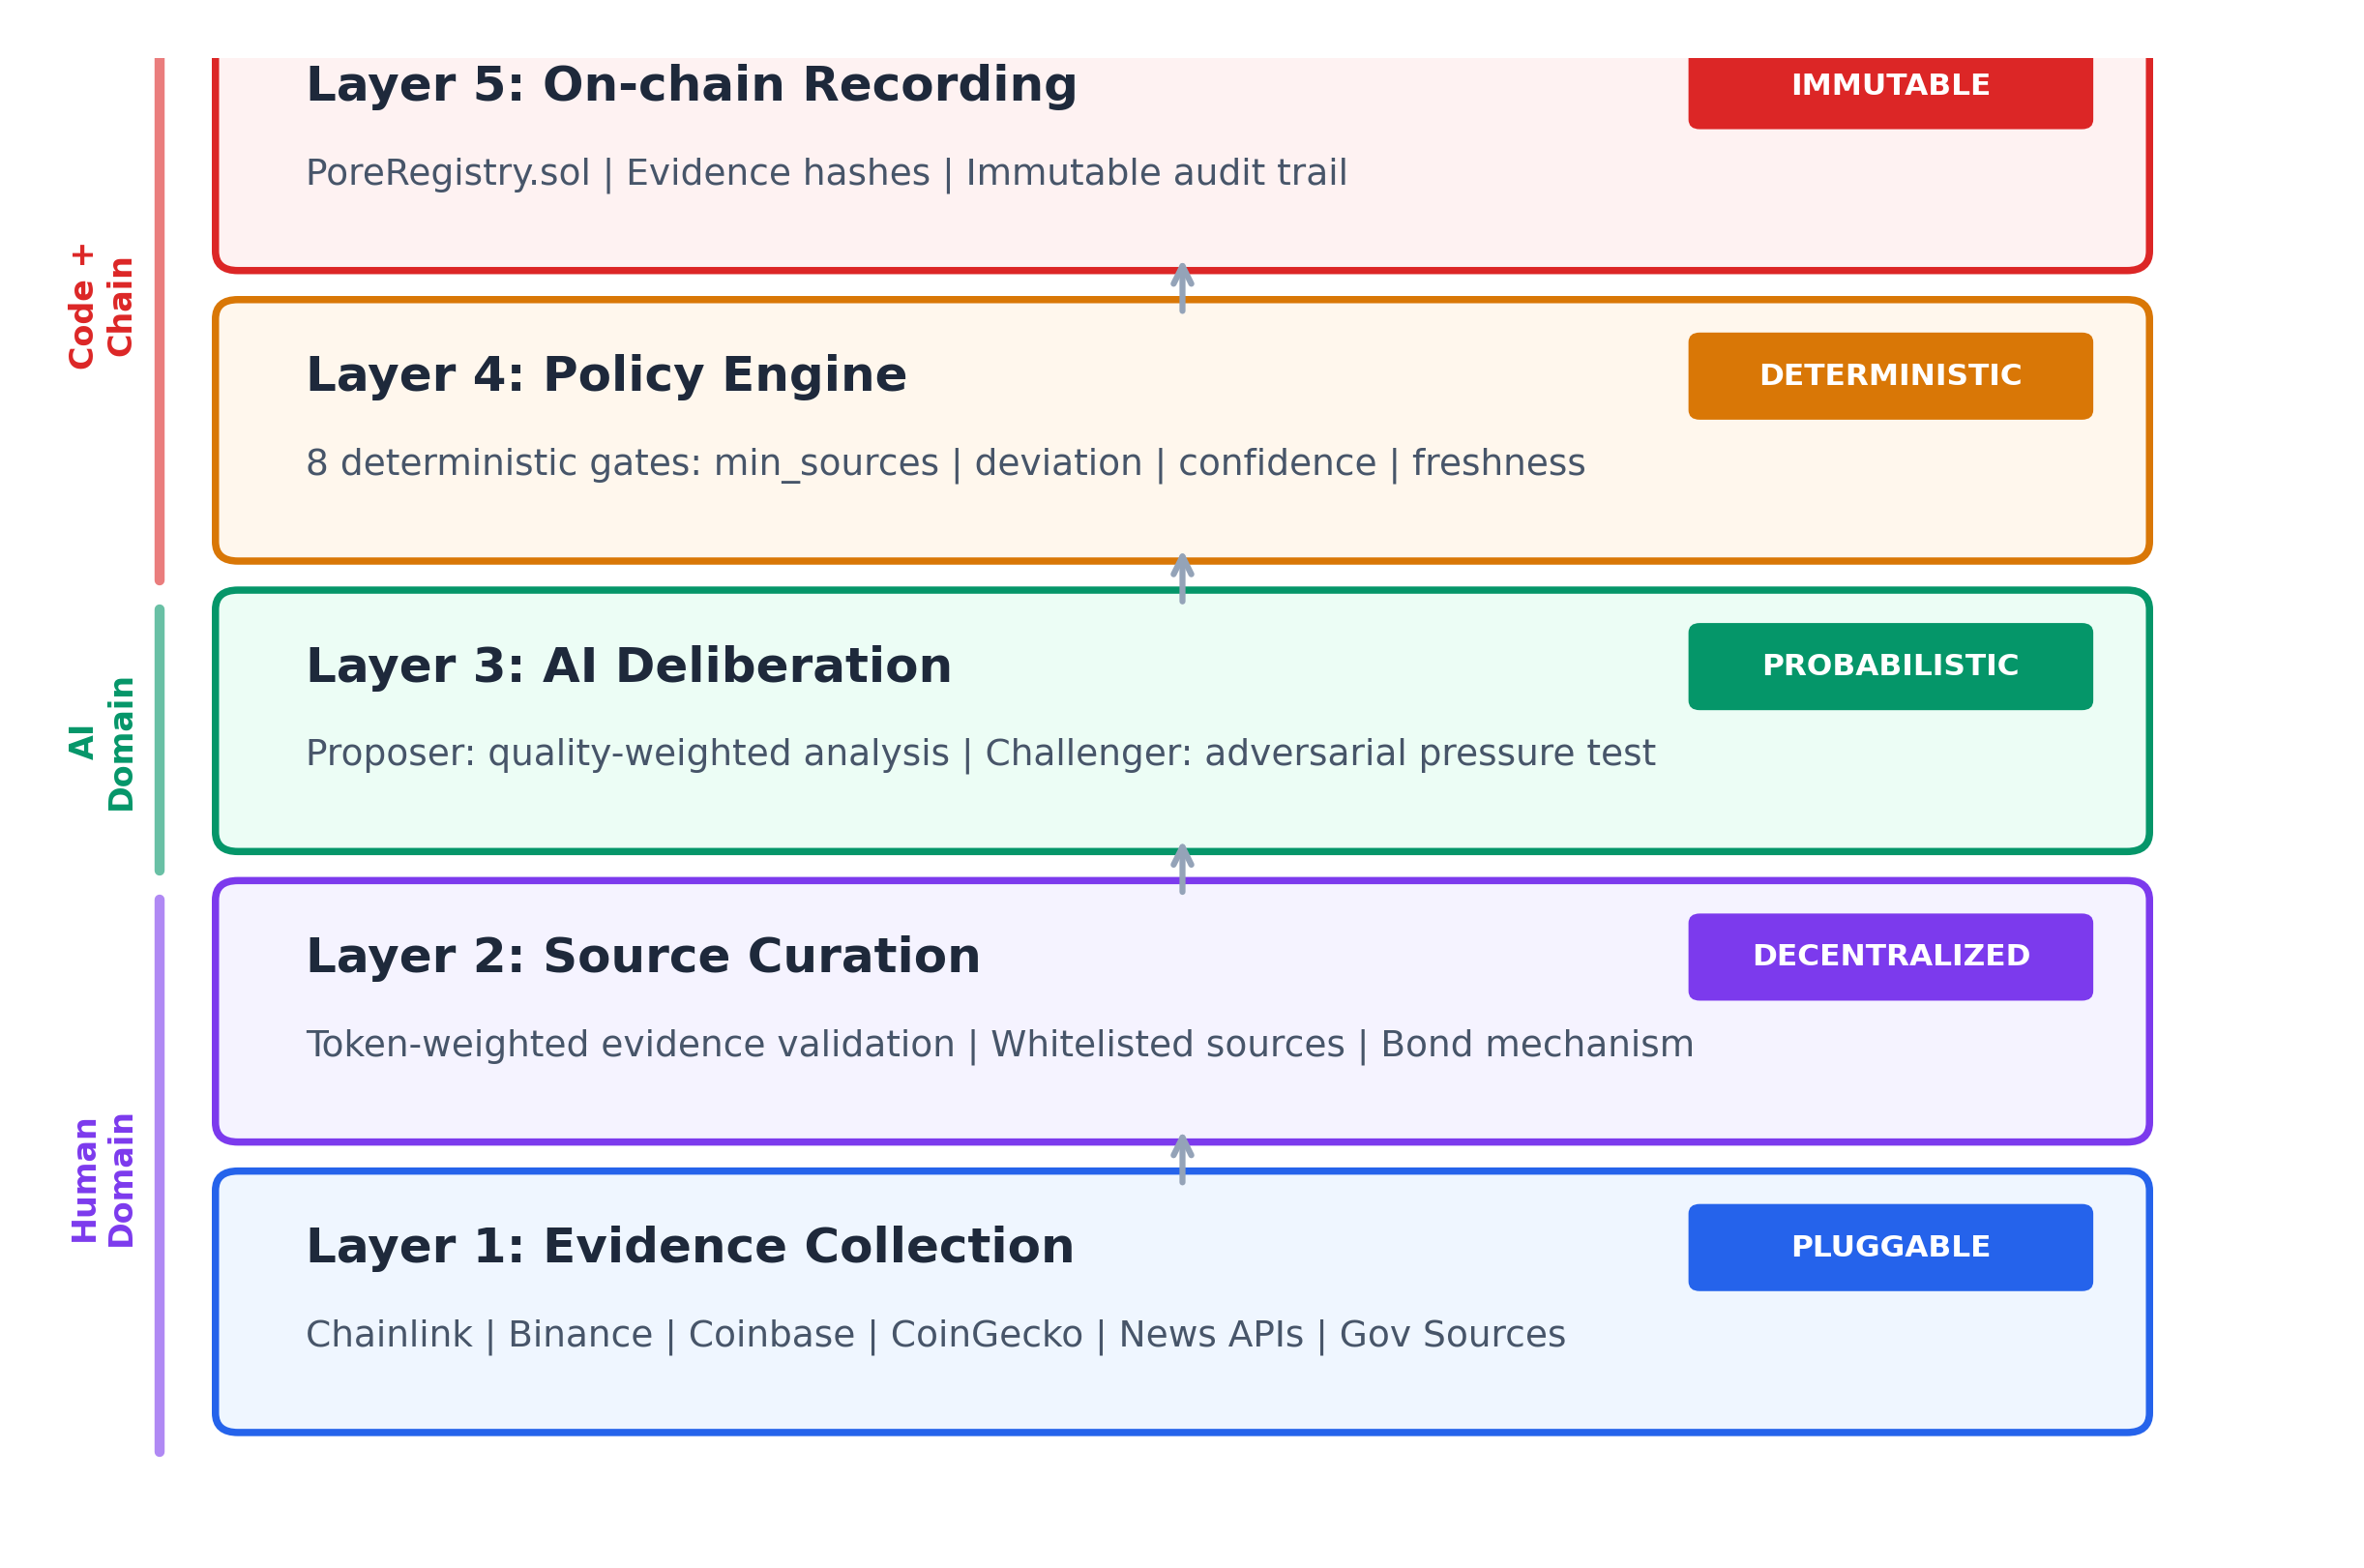
\includegraphics[width=0.88\textwidth]{diagrams/fig1_architecture.png}
    \caption{PoRE five-layer architecture. Trust domains: humans curate evidence (L1--2), AI interprets (L3), code evaluates safety (L4), blockchain records (L5).}
    \label{fig:arch}
\end{figure*}
\FloatBarrier

\subsection{State Machine}

Each resolution progresses through defined states (Figure~\ref{fig:sm}):
\begin{multline*}
\textsc{pending} \to \textsc{proposed} \to \textsc{challenged} \\
\to \{\textsc{acc.}/\textsc{rej.}\}
\xrightarrow{\pi} \{\textsc{auto}/\textsc{hold}\}
\end{multline*}

\begin{figure*}[!htbp]
    \centering
    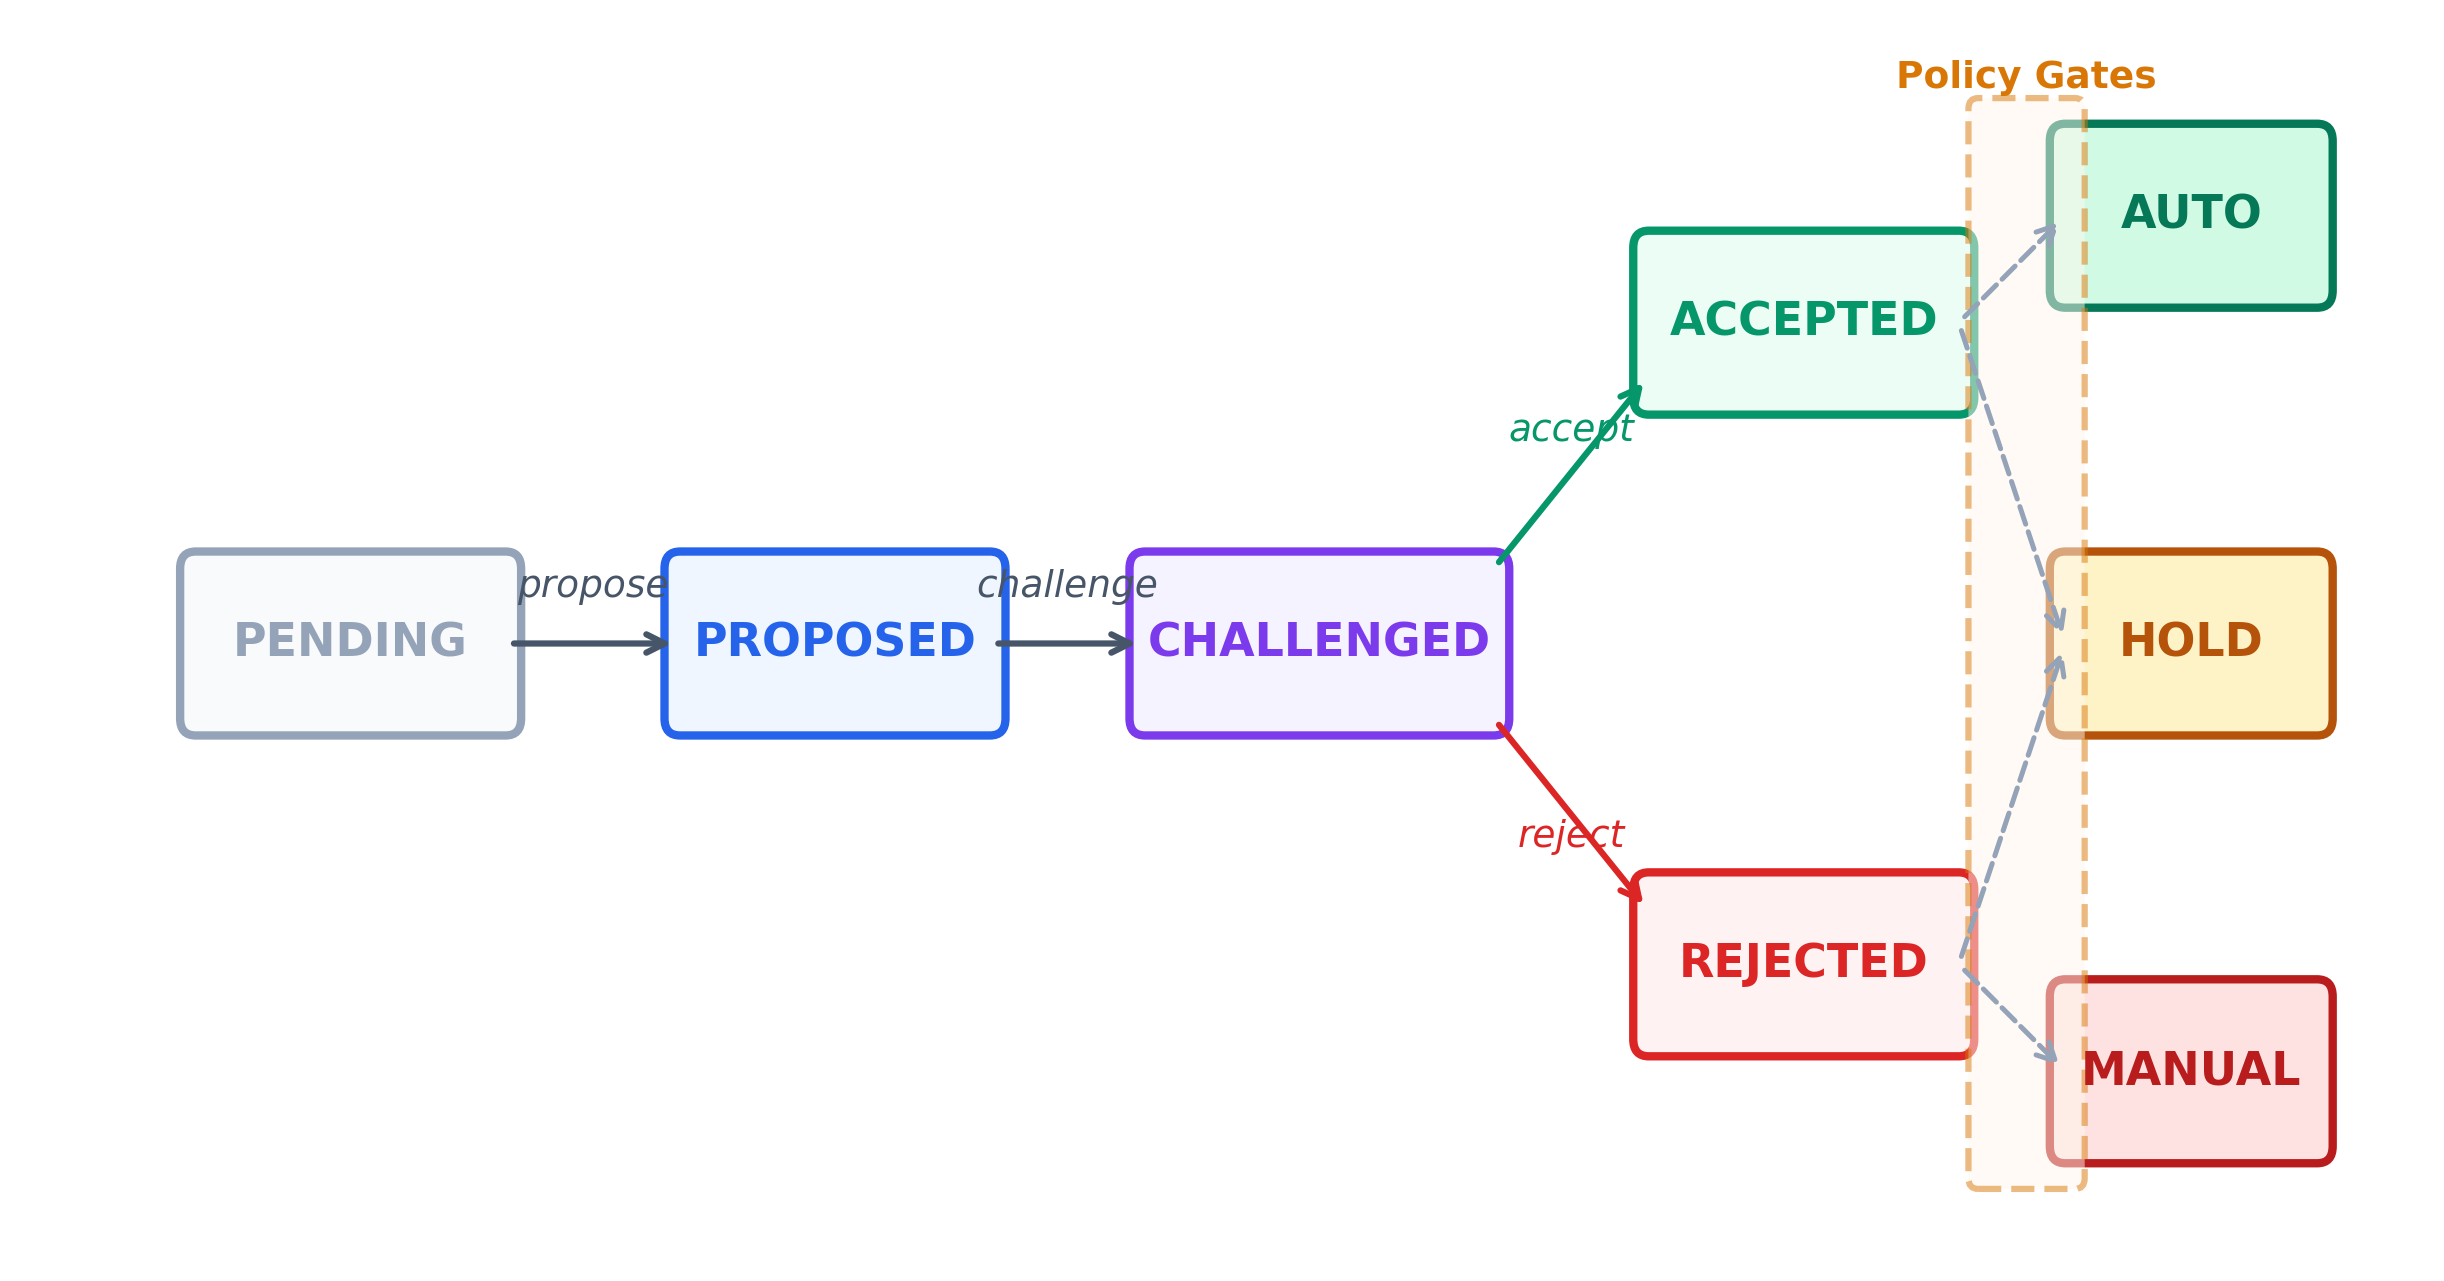
\includegraphics[width=0.82\textwidth]{diagrams/fig2_state_machine.png}
    \caption{State machine. Policy gates (dashed) are the final safety barrier. All transitions are deterministic and logged.}
    \label{fig:sm}
\end{figure*}
\FloatBarrier

\subsection{Evidence Schema}

Each evidence item $e_i$ is a tuple:
\begin{equation}
    e_i = (s_i,\; \tau_i \in \mathcal{T},\; q_i \in [0,1],\; v_i \in [0,1],\; h_i)
    \label{eq:evidence}
\end{equation}
where $s_i$ is the source, $\tau_i$ is the type, $q_i$ is quality, $v_i$ is the YES-signal, and $h_i$ is the SHA-256 hash.

% ═══════════════════════════════════════════════════
\section{Deterministic Policy Engine}

The policy engine is the \emph{trust anchor}---deterministic code, not AI. Given identical inputs, it produces identical outputs.

\subsection{Policy Parameters}

A policy $\pi$ defines:
\begin{equation}
    \pi = (n_{\min},\; t_{\min},\; \delta_{\max},\; \gamma_{\min},\; \alpha_{\max})
    \label{eq:policy}
\end{equation}
where $n_{\min}$ = min sources, $t_{\min}$ = min source types, $\delta_{\max}$ = max deviation, $\gamma_{\min}$ = confidence threshold, $\alpha_{\max}$ = max evidence age (hours).

\subsection{Evaluation Algorithm}

\begin{algorithm}[H]
\caption{Policy Evaluation}
\label{alg:policy}
\footnotesize
\begin{algorithmic}[1]
\Require Evidence $E = \{e_1,\ldots,e_n\}$, policy $\pi$
\Ensure Verdict, violation set $V$
\State $V \gets \emptyset$
\If{$|E| < n_{\min}$}
    \State $V \gets V \cup \{\texttt{MIN\_SRC}\}$
\EndIf
\If{$|\{\tau_i\}| < t_{\min}$}
    \State $V \gets V \cup \{\texttt{TYPE\_DIV}\}$
\EndIf
\State $\bar{v} \gets \sum_i q_i v_i \;/\; \sum_i q_i$
\Comment{Weighted mean}
\State $\sigma \gets \sqrt{\sum_i q_i(v_i - \bar{v})^2 \;/\; \sum_i q_i}$
\If{$\sigma > \delta_{\max}$}
    \State $V \gets V \cup \{\texttt{DEVIATION}\}$
\EndIf
\State $\gamma \gets f(\sigma, E)$
\Comment{Eq.~\ref{eq:conf}}
\If{$\gamma < \gamma_{\min}$}
    \State $V \gets V \cup \{\texttt{LOW\_CONF}\}$
\EndIf
\If{$V = \emptyset$}
    \Return \textsc{auto}
\Else{}
    \Return \textsc{hold}, $V$
\EndIf
\end{algorithmic}
\end{algorithm}

\subsection{Confidence Score}

\begin{equation}
    \gamma = w_1(1{-}\sigma) + w_2 \frac{|\mathcal{T}_E|}{|\mathcal{T}|} + w_3 \!\left(1 {-} \frac{\max_i \text{age}(e_i)}{\alpha_{\max}}\right)
    \label{eq:conf}
\end{equation}
with default weights $(w_1,w_2,w_3) = (0.5, 0.3, 0.2)$.

\subsection{Why Not AI?}

LLMs are stochastic (different outputs for identical inputs), unauditable (``the AI felt insufficient'' is not verifiable), and adversarially vulnerable (prompt injection). The inequality $\sigma > 0.30$ is verifiable by anyone, always.

% ═══════════════════════════════════════════════════
\section{Decentralized Source Curation}

This section presents the primary novel contribution.

\subsection{Core Idea}

Current systems: token holders vote on outcomes (1-bit). We propose voting on \emph{evidence validity}:
\begin{align*}
\text{UMA:}\quad & \text{voters} \xrightarrow{\text{vote}} \{\textsc{yes},\textsc{no}\} \\
\text{PoRE:}\quad & \text{voters} \xrightarrow{\text{curate}} E' \xrightarrow{\text{engine}} \text{verdict}
\end{align*}

\subsection{Protocol Phases}

Five phases (Figure~\ref{fig:curation}):
\begin{enumerate}[nosep]
    \item \textbf{Submission} (24h): anyone submits with bond $b$.
    \item \textbf{Voting} (48h): token-weighted \textsc{valid}/\textsc{invalid}. Whitelisted types $\mathcal{W}$ cannot be excluded.
    \item \textbf{AI Analysis}: proposer + challenger.
    \item \textbf{Policy Engine}: Algorithm~\ref{alg:policy}.
    \item \textbf{Resolution}: \textsc{auto} or \textsc{hold}.
\end{enumerate}

\begin{figure*}[!htbp]
    \centering
    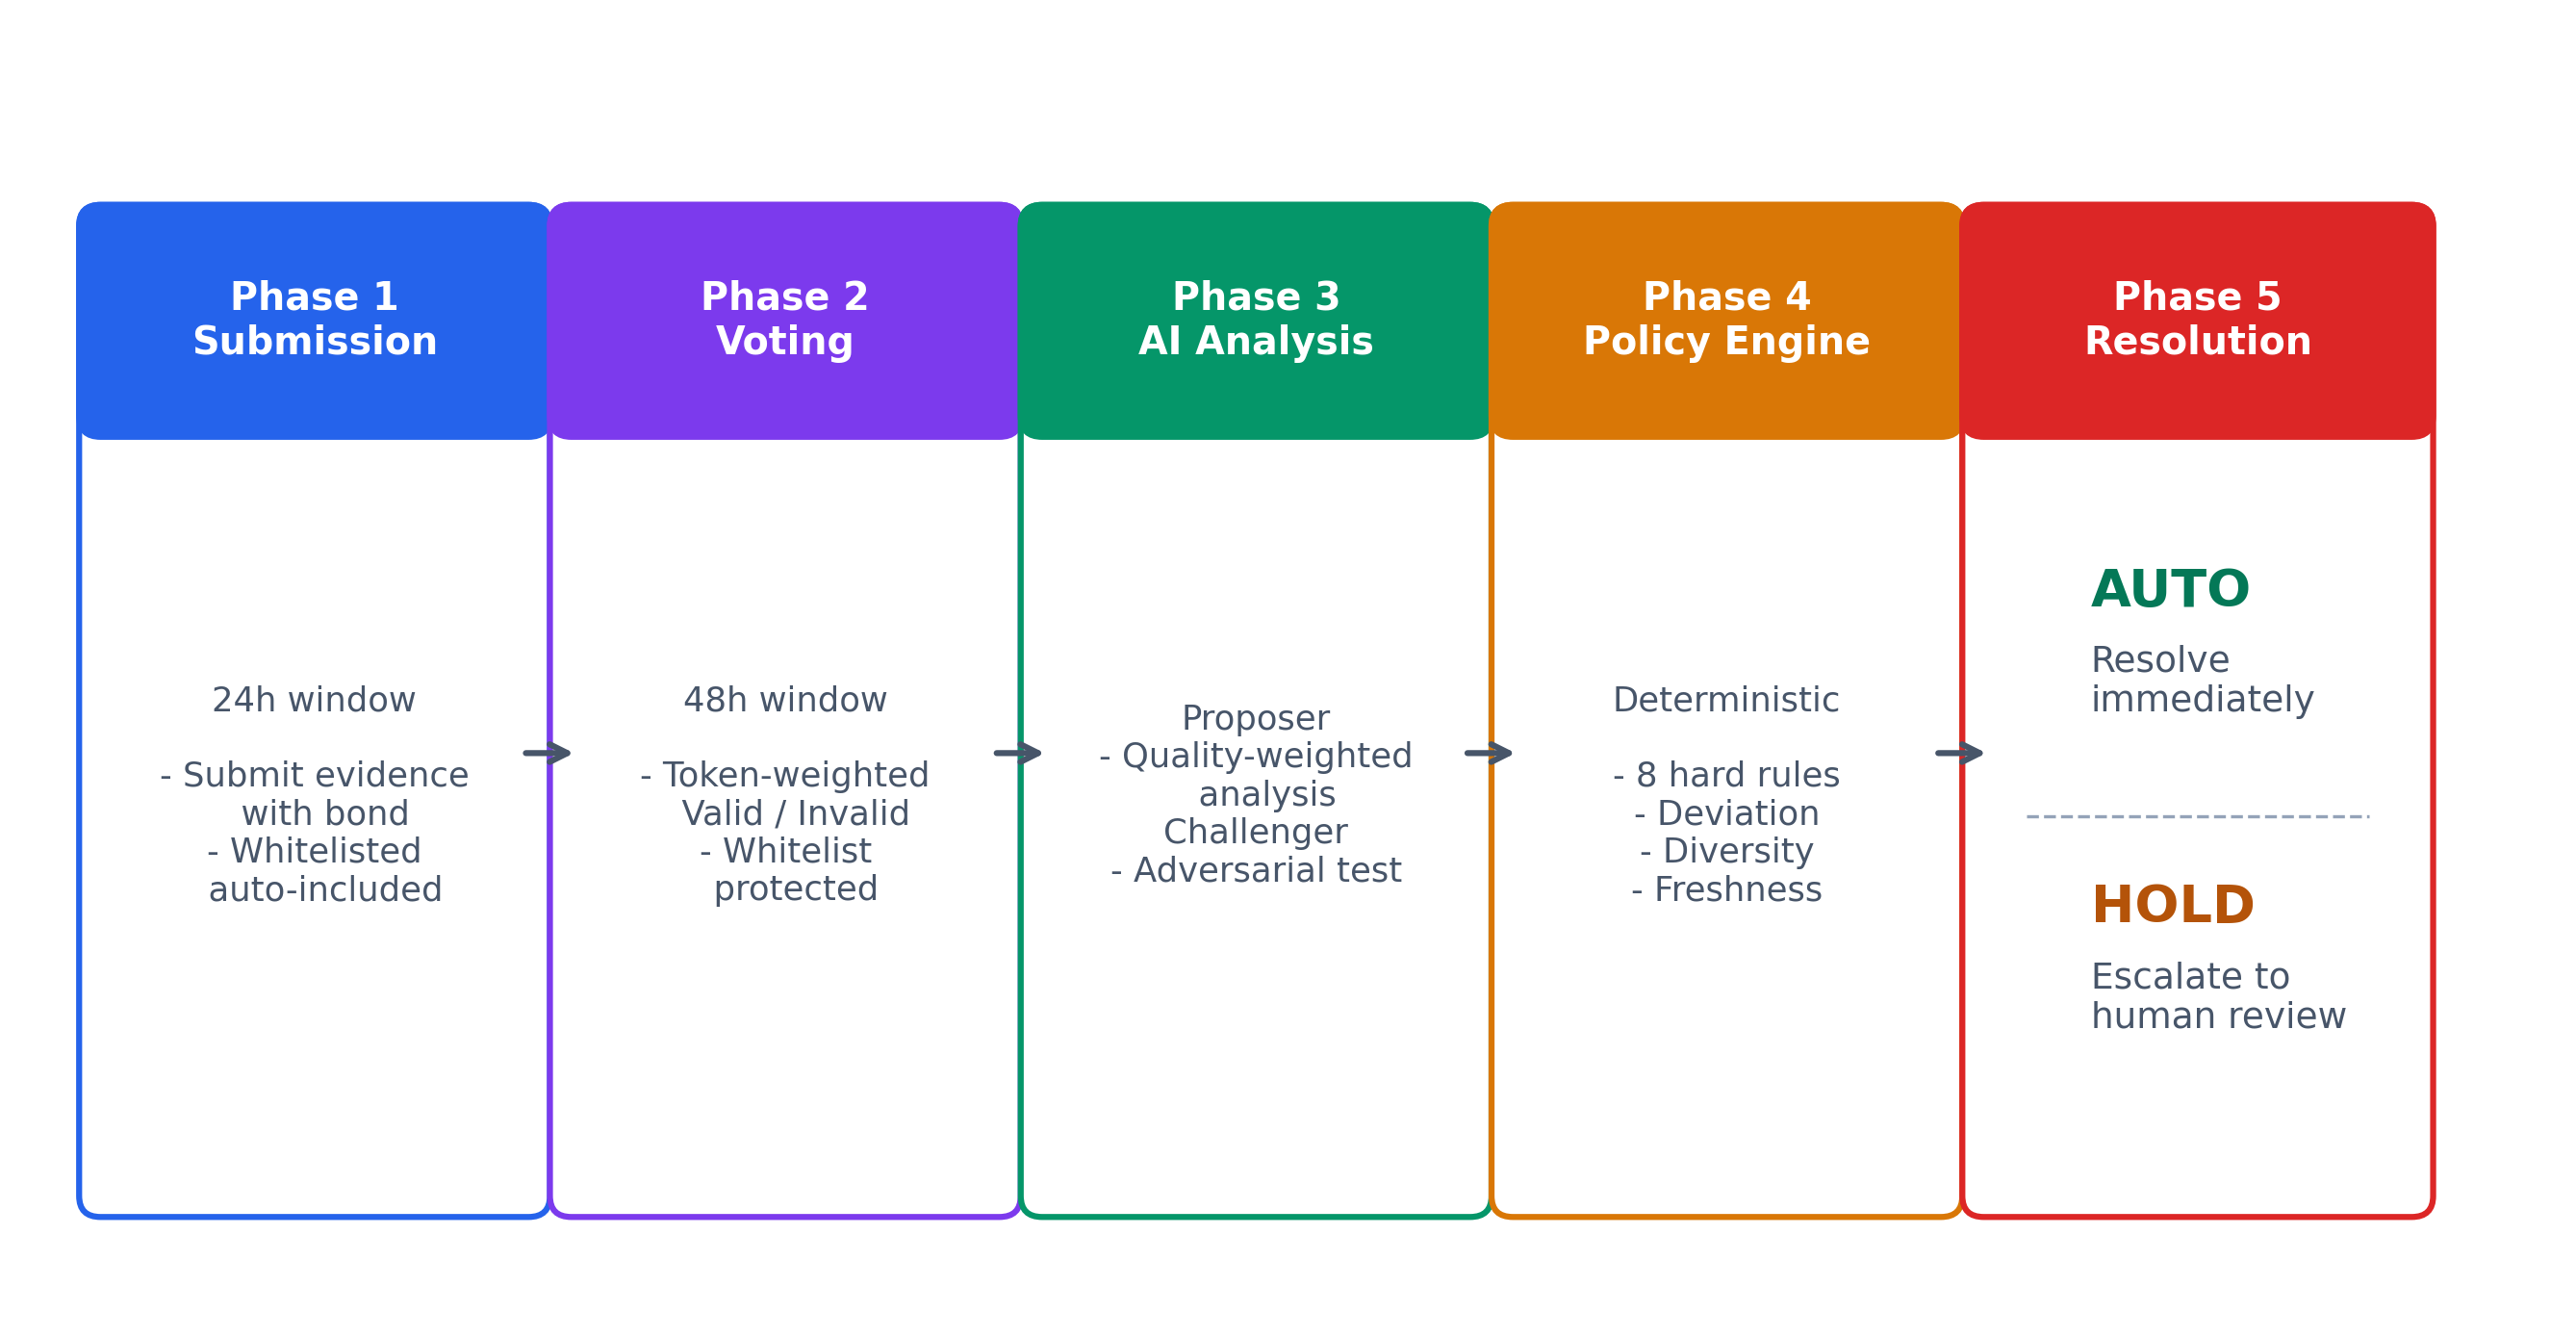
\includegraphics[width=0.88\textwidth]{diagrams/fig3_source_curation.png}
    \caption{Decentralized Source Curation protocol. Token-weighted validation (Phase~2) feeds into deterministic policy evaluation (Phase~4).}
    \label{fig:curation}
\end{figure*}
\FloatBarrier

\subsection{Quality Scoring}

Base quality $q_0(\tau)$ (Table~\ref{tab:quality}) is adjusted by vote ratio $r_i$:
\begin{equation}
    q_i = q_0(\tau_i) \cdot (0.8 + 0.4 \cdot r_i)
    \label{eq:qadj}
\end{equation}

Even with unanimous support ($r_i=1$):
\begin{equation}
    q_{\texttt{social}} = 0.20 \times 1.20 = 0.24 \ll 0.95 = q_{\texttt{oracle}}
    \label{eq:cap}
\end{equation}

\begin{table}[h]
\centering
\caption{Base quality by source type.}
\label{tab:quality}
\footnotesize
\begin{tabular}{@{}lr@{}}
\toprule
\textbf{Source Type} & $q_0$ \\
\midrule
\texttt{onchain\_oracle} & 0.95 \\
\texttt{official\_govt} & 0.95 \\
\texttt{news\_agency} & 0.85 \\
\texttt{cex\_spot} & 0.75 \\
\texttt{aggregator} & 0.60 \\
\texttt{image\_analysis} & 0.50 \\
\texttt{social\_media} & 0.20 \\
\bottomrule
\end{tabular}
\end{table}

\subsection{Whitelist Mechanism}

Types $\mathcal{W} = \{\texttt{official\_govt},\, \texttt{onchain\_oracle}\}$ cannot be excluded by vote. If the State Dept publishes ``No deal,'' this source persists regardless of token holder preferences.

\subsection{Anti-Manipulation}

\textbf{Flooding}: bond per submission, deduplication, type diversity rule, quality ceiling. \textbf{Removal}: whitelist, exclusion metadata, min source count. \textbf{Sybil}: token-weighted voting inherently resists sybil. \textbf{Collusion}: policy engine independently checks all constraints.

% ═══════════════════════════════════════════════════
\section{Game-Theoretic Analysis}

\subsection{Attack Cost}

Under UMA (Figure~\ref{fig:attack}a):
\begin{equation}
    C_A = \max\!\left(b,\; \frac{n_{\text{maj}} \cdot p_{\text{tok}}}{\text{participation}}\right) \approx \$10.5\text{M}
    \label{eq:ca}
\end{equation}

Under PoRE, the attacker must satisfy constraints (\ref{eq:c1})--(\ref{eq:c5}) simultaneously:
\begin{align}
    |E'| &\geq n_{\min} \label{eq:c1} \\
    |\mathcal{T}_{E'}| &\geq t_{\min} \label{eq:c2} \\
    \sigma(E') &\leq \delta_{\max} \label{eq:c3} \\
    \gamma(E') &\geq \gamma_{\min} \label{eq:c4} \\
    \forall\, e_w \in \mathcal{W}&:\; e_w \in E' \label{eq:c5}
\end{align}

Constraint~(\ref{eq:c5}) is decisive: whitelisted sources reflecting ground truth cannot be removed. When they contradict the desired outcome, satisfying~(\ref{eq:c3})--(\ref{eq:c4}) is infeasible:
\begin{equation}
    C_B \to \infty
    \label{eq:cb}
\end{equation}

\subsection{Dimensionality}

\begin{table}[h]
\centering
\caption{Manipulation dimensionality.}
\label{tab:dim}
\footnotesize
\begin{tabular}{@{}llc@{}}
\toprule
\textbf{System} & \textbf{Target} & \textbf{Dim.} \\
\midrule
UMA & YES/NO & 1 bit \\
Kleros & Juror verdicts & $N$ bits \\
Augur & Dispute bonds & Sequential \\
\textbf{PoRE} & \textbf{Evidence set} & $\mathbf{N \!\times\! |\mathcal{T}| \!\times\! \mathbb{R}^3}$ \\
\bottomrule
\end{tabular}
\end{table}

\begin{figure*}[!htbp]
    \centering
    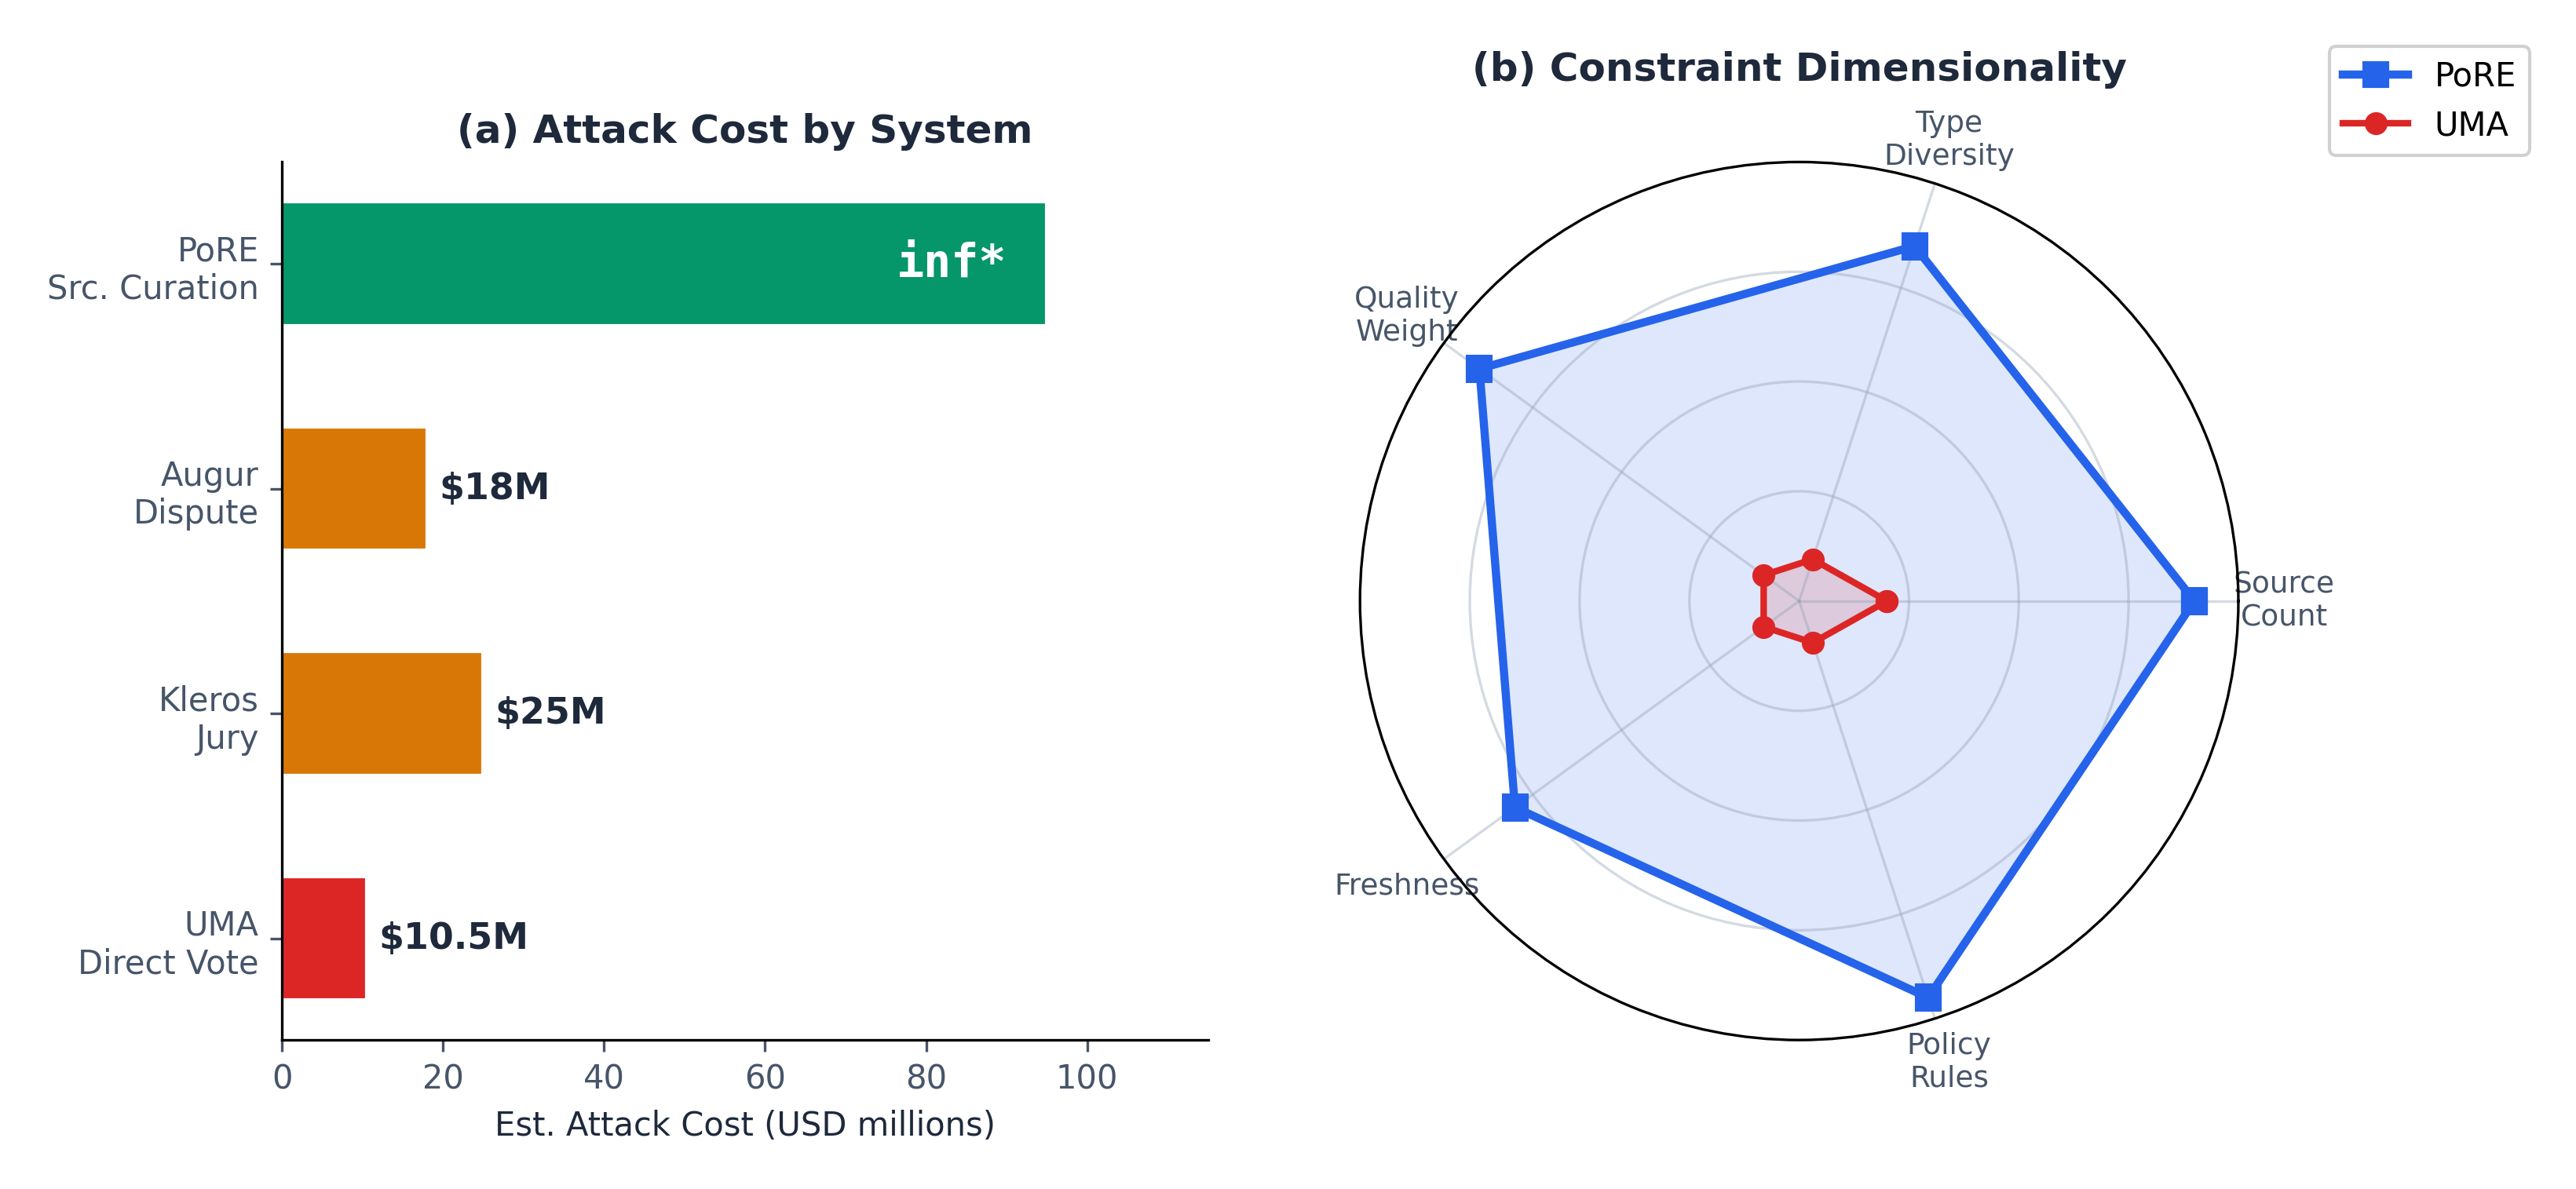
\includegraphics[width=0.88\textwidth]{diagrams/fig4_attack_cost.png}
    \caption{(a)~Attack cost comparison. PoRE with whitelisted sources is structurally infeasible. (b)~Constraint dimensionality radar.}
    \label{fig:attack}
\end{figure*}
\FloatBarrier

\subsection{Nash Equilibrium}

The \textbf{honest equilibrium} is dominant: voters validate truthfully, clear cases resolve via \textsc{auto}, ambiguous cases escalate. The manipulation equilibrium is unstable: high cost, uncertain success, and full traceability (excluded sources logged on-chain).

% ═══════════════════════════════════════════════════
\section{Case Studies}

\subsection{Ukraine Mineral Deal (\$7M)}

A whale (${\sim}5$M UMA, ${\sim}25\%$ voting) forced YES with no official confirmation. PoRE replay at $T{+}1$h (Figure~\ref{fig:case}):

Quality-weighted average:
\begin{align}
    \bar{v} &= \frac{\sum_i q_i v_i}{\sum_i q_i} \nonumber \\
    &= \frac{0.095 {+} 0.143 {+} 0.180 {+} 0.170 {+} 0.158}{3.85} \nonumber \\
    &= 0.194 \quad (\text{NO})
    \label{eq:ukraine}
\end{align}

Deviation $\sigma = 0.43 > 0.30$. Five violations. \textbf{Verdict: \textsc{hold}.}

Under source curation, State Dept and Ukraine MFA are whitelisted ($q=0.95$), dominating the weighted average. Even flooding with social media ($q_{\max}=0.24$) cannot shift~$\bar{v}$.

\begin{figure*}[!htbp]
    \centering
    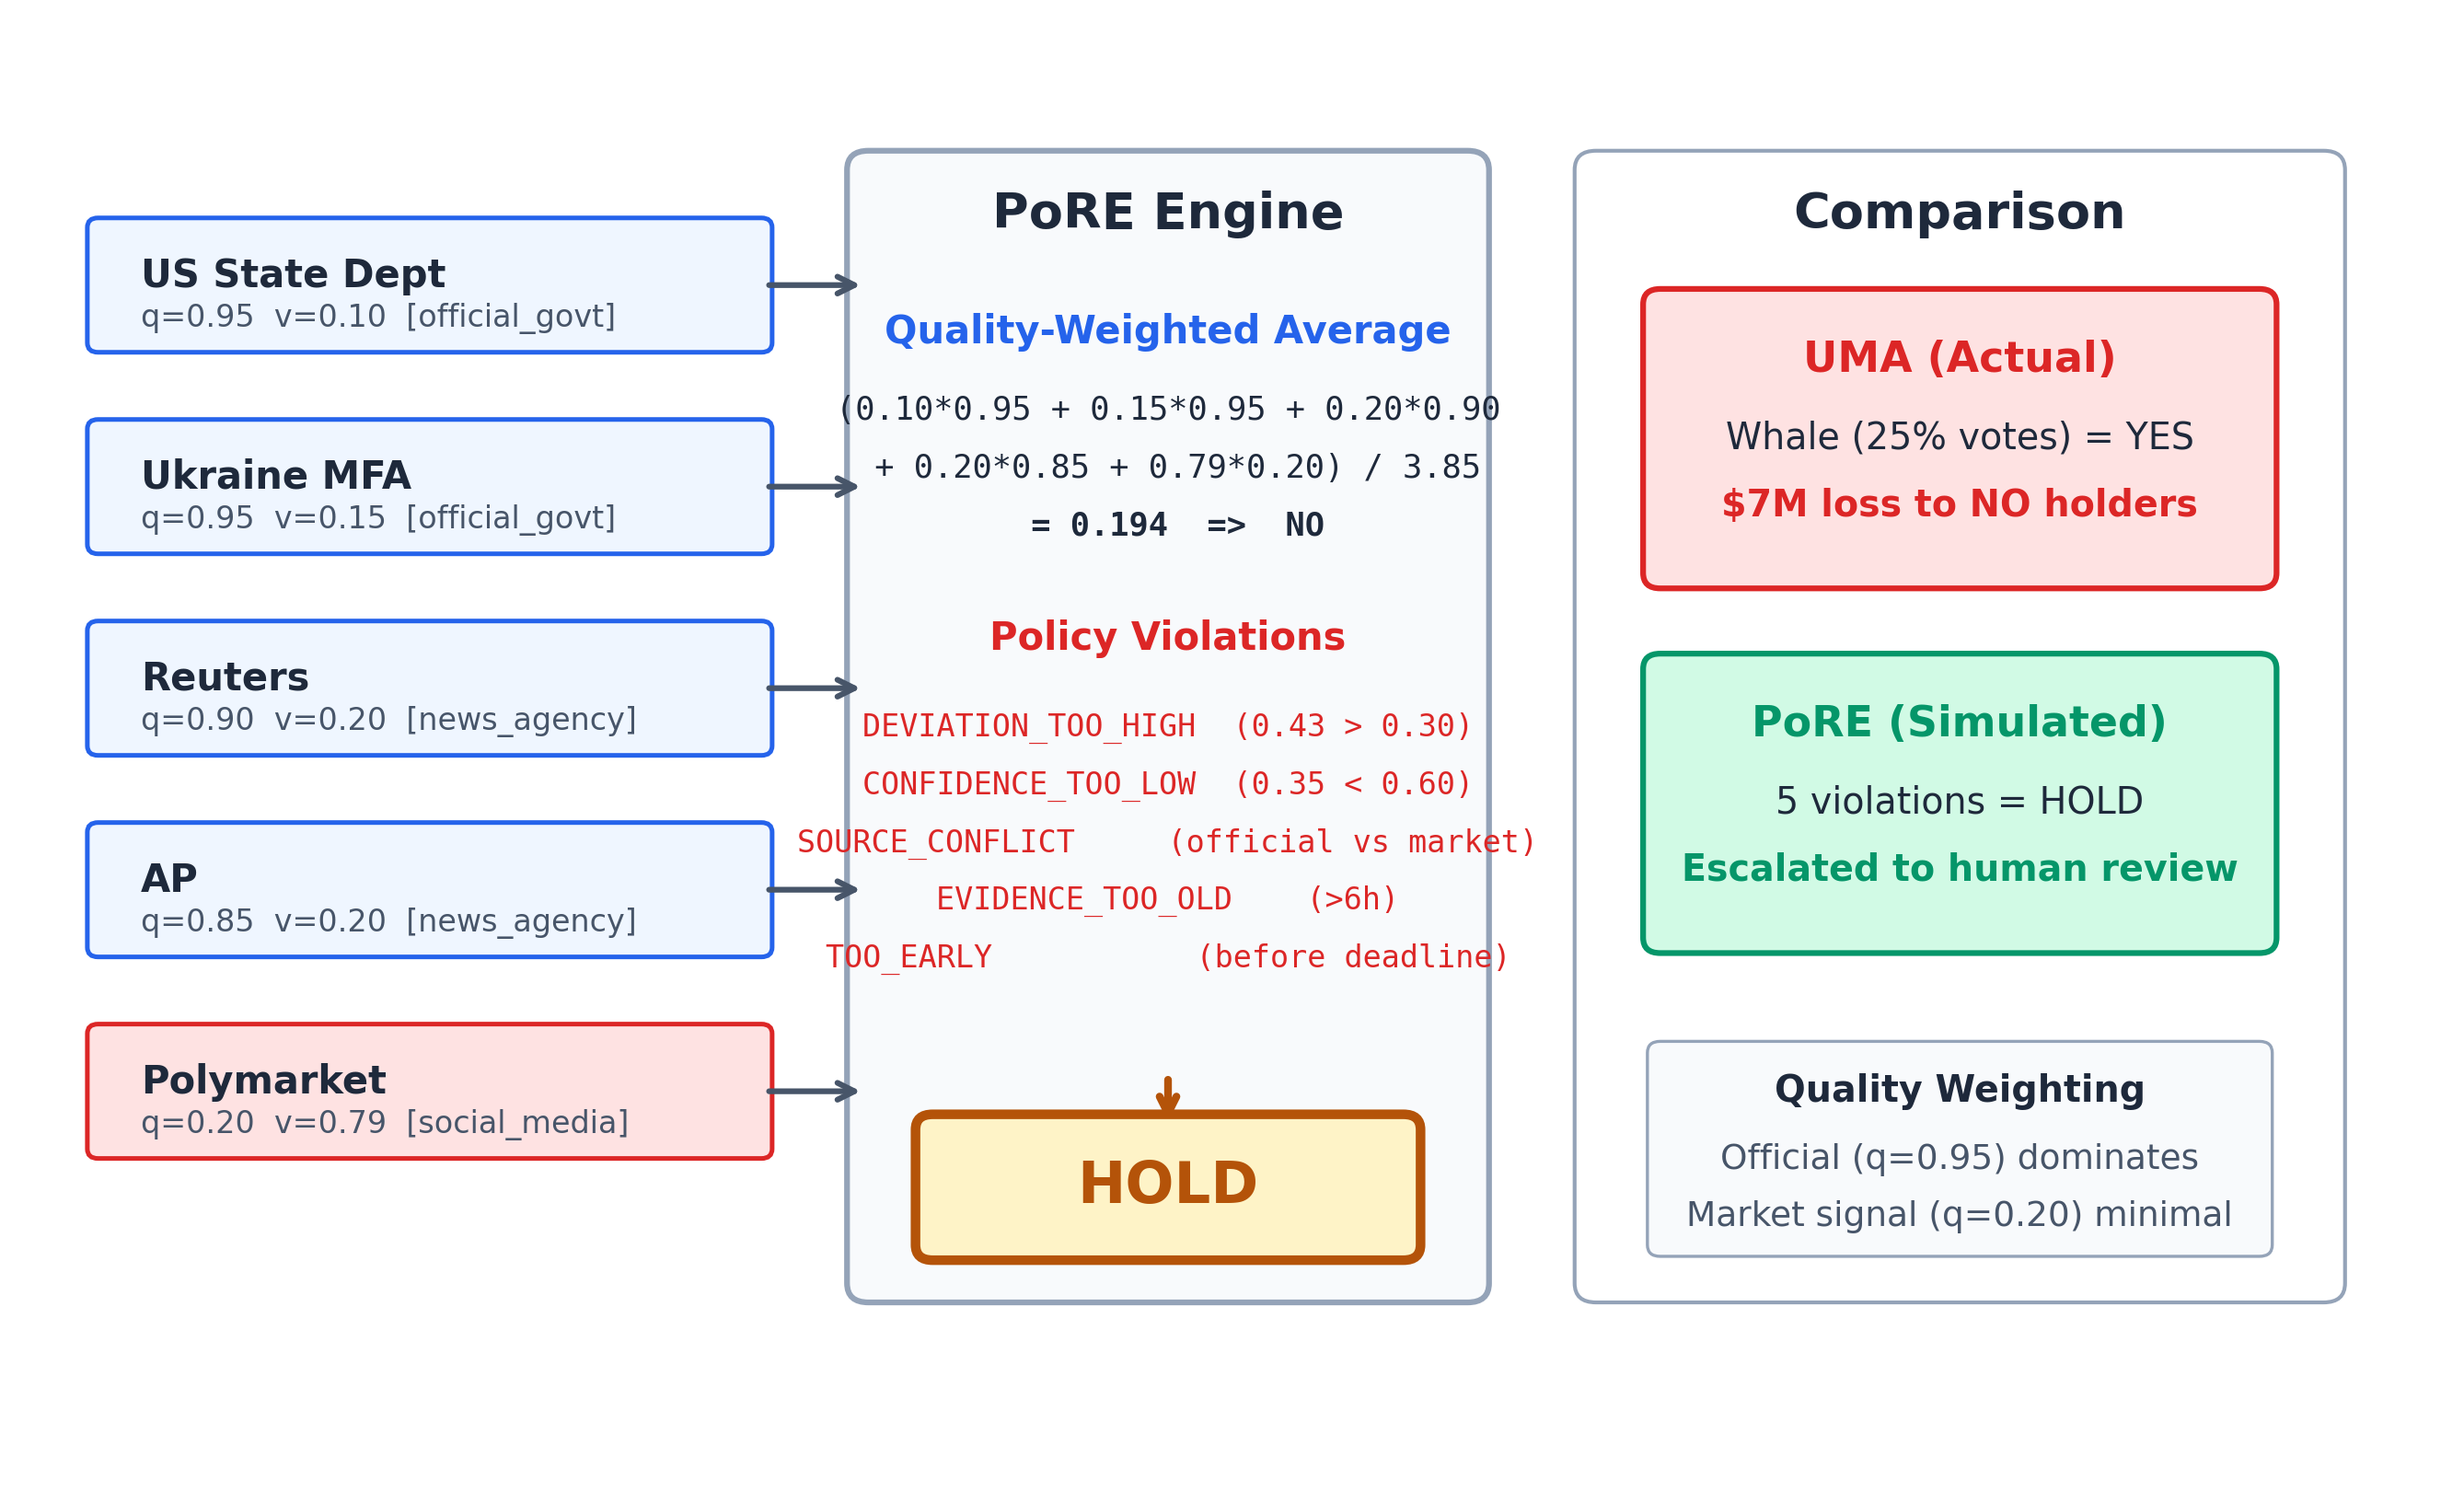
\includegraphics[width=0.85\textwidth]{diagrams/fig5_case_study.png}
    \caption{Ukraine mineral deal case. Official sources ($q{=}0.95$) dominate the weighted average, producing five violations and \textsc{hold}. UMA resolved YES via whale voting (\$7M loss).}
    \label{fig:case}
\end{figure*}
\FloatBarrier

\subsection{Zelenskyy Suit (\$237M)}

Photo evidence from Reuters/AP/Getty, but two whales resolved NO. PoRE: $\bar{v}=0.718$ (YES-leaning), $\sigma=0.38>0.30$. Source type conflict. \textbf{Verdict: \textsc{hold}.} Correct---genuinely ambiguous.

% ═══════════════════════════════════════════════════
\section{Implementation}

The prototype is JavaScript (Node.js), zero dependencies beyond \texttt{ethers}:

\begin{table}[h]
\centering
\caption{Core modules.}
\label{tab:modules}
\footnotesize
\begin{tabularx}{\columnwidth}{@{}lX@{}}
\toprule
\textbf{Module} & \textbf{Function} \\
\midrule
\texttt{policy/evaluator} & Deterministic engine \\
\texttt{ai/proposer} & Quality-weighted analysis \\
\texttt{ai/challenger} & Adversarial challenge \\
\texttt{evidence/chainlink} & Mainnet price feed \\
\texttt{evidence/liveCollect} & 4-source real-time \\
\texttt{workflow/onchain} & On-chain recording \\
\texttt{PoreRegistry.sol} & Solidity registry \\
\bottomrule
\end{tabularx}
\end{table}

Live evaluation collects from Chainlink BTC/USD (Ethereum mainnet), Binance, Coinbase, and CoinGecko. All 9~tests pass; self-score~100/High.

% ═══════════════════════════════════════════════════
\section{Discussion}

\textbf{Limitations.} Evidence collection for subjective events uses pre-curated data; production needs automated pipelines. Base quality scores are expert-assigned; empirical calibration is future work. Policy parameter governance itself requires a mechanism.

\textbf{vs.\ Pure AI.} A well-prompted LLM approximates PoRE \emph{most of the time}. For \$237M, ``most'' is insufficient. LLMs are stochastic, unauditable, and adversarially vulnerable. PoRE's policy layer is code: same input, same output, always.

% ═══════════════════════════════════════════════════
\section{Future Work}

\begin{enumerate}[nosep]
    \item Smart contract for source curation voting.
    \item Empirical quality calibration from historical data.
    \item Cross-platform federation (Polymarket, Kalshi, Augur).
    \item Formal verification of policy engine properties.
    \item Proof-of-personhood hybrid voting (World~ID).
\end{enumerate}

% ═══════════════════════════════════════════════════
\section{Conclusion}

Prediction markets need a system that knows \emph{when it doesn't know}. PoRE introduces a deterministic policy engine that cannot be manipulated, and a source curation protocol shifting manipulation from 1-bit corruption to $N$-dimensional constraint satisfaction. In replays of \$247M+ in failures, PoRE produced \textsc{hold} in every case.

The oracle problem is solved not by more powerful AI or larger token stakes, but by architectural separation: AI interprets, code enforces, humans arbitrate, blockchain records.

% Figures are placed inline near their references via \FloatBarrier

% ═══════════════════════════════════════════════════
\begin{thebibliography}{10}

\bibitem{wolfers2004prediction}
J.~Wolfers and E.~Zitzewitz, ``Prediction Markets,'' \emph{J.~Econ.~Perspectives}, 18(2):107--126, 2004.

\bibitem{chainlink2021}
L.~Breidenbach et~al., ``Chainlink 2.0,'' Chainlink Whitepaper, 2021.

\bibitem{uma2020}
A.~Hart et~al., ``UMA: Universal Market Access,'' UMA Whitepaper, 2020.

\bibitem{kleros2017}
F.~Ast and B.~Deffains, ``Kleros,'' Kleros Whitepaper, 2017.

\bibitem{augur2015}
J.~Peterson et~al., ``Augur,'' Augur Whitepaper, 2015.

\bibitem{api3}
API3, ``Decentralized APIs for Web 3.0,'' 2020.

\bibitem{olas2023}
Olas Network, ``Autonolas,'' Olas Documentation, 2023.

\bibitem{buterin2014}
V.~Buterin, ``Ethereum Whitepaper,'' 2014.

\bibitem{polymarket2024}
Polymarket Documentation, 2024.

\bibitem{arrow1970}
K.~J.~Arrow, \emph{Essays in the Theory of Risk-Bearing}, North-Holland, 1970.

\end{thebibliography}

\end{document}
